\documentclass{article}

\usepackage[margin=1in]{geometry}
\usepackage{color}
\usepackage{hyperref}
\usepackage{soul}
\usepackage{float}
\usepackage{amsmath}

\usepackage[sc]{mathpazo}
\linespread{1.20}         % Palatino needs more leading (space between lines)
\usepackage[T1]{fontenc}
\usepackage{microtype}
\usepackage{listings}
\usepackage{courier}
\usepackage{graphicx}
\usepackage{caption}
\usepackage{subcaption}

\definecolor{mygreen}{rgb}{0,0.6,0}
\definecolor{light-gray}{gray}{0.95}

\lstset{basicstyle=\footnotesize\ttfamily,breaklines=true,language=Prolog}
\lstset{frame=single,commentstyle=\color{mygreen}}
\lstset{aboveskip=0.5cm,belowskip=0.3cm}
\lstset{backgroundcolor=\color{light-gray}}

\hypersetup{pdfpagemode=UseNone}

\newcommand{\manager}{\texttt{manager} }
\newcommand{\eagent}{\texttt{elevator agent} }
\newcommand{\eagents}{\texttt{elevator agents} }
\newcommand{\todo}[1] {\hl{TODO: #1}}
\newcommand{\horrule}[1]{\rule{\linewidth}{#1}}
\setlength{\parindent}{0cm}

\title{ 	
		\usefont{OT1}{bch}{b}{n}
		\normalfont \normalsize \textsc{Delft University of Technology \protect\\ Data Visualization 2015 - 2016} \\ [25pt]
		\horrule{0.5pt} \\[0.4cm]
		\huge Football Match Visualization Project \\
		Individual Report
		\horrule{2pt} \\[0.5cm]
}
\author{
		\normalfont 								\normalsize
        Overvoorde Alexander 4153235\\[-3pt]		\normalsize
        \today
}
\date{}
\begin{document}
\lstset{language=sql}
\maketitle

\newpage
\section{3D visualization}

I wrote a Python script that took the position, energy and speed data and generated team and per-player heatmaps from these as 2D grids with values scaled from 0 to 1. These are stored as arrays in JSON format. I visualized these with three.js (figure \ref{fig:3dvis}) by creating a plane and deforming it based on the heatmap value. The color is calculated using a d3.js scale. I created the field models (pitch, goals) with Blender. I implemented the camera movement by taking the code from the three.js OrbitControls example.
\\ \\
The players are simply cube geometry and are positioned based on the interpolated positions in the 2D visualization. They are also rotated based on the direction of the player. To make this work properly with the transitions I implemented a custom \verb#attrTween# function that finds the shortest angle so that a player rotating from 350 degrees to 5 degrees doesn't turn all the way around.
\\
Player selection is implemented by assigning the ID to each player mesh as JavaScript object property and using a raycast to find which player is under the cursor when the user clicks.

\section{2D visualization}

I developed the 2D visualization (figure \ref{fig:2dvis}) with d3.js and wrote the code for the playback controls and heatmap selection. The heatmap selection toggles the visibility of the generated heatmap meshes in the 3D visualization. The play/pause button and playback speed selector modifies the frequency of a \verb#setInterval# timer that loads the next frame of player positions. The updates use d3.js transitions to make movement appear smoothly.
\\ \\
The frame data originates from a CSV file that is loaded with an AJAX request. The CSV contains the position, energy and speed per player per second. I generated it by importing the source data in PostgreSQL and exporting only the per-second data with the following query:

\begin{lstlisting}
SELECT DISTINCT ON (DATE_TRUNC('sec', timestamp), tag_id) *, DATE_TRUNC('sec', timestamp) AS t FROM positions;
\end{lstlisting}

\begin{figure}[ht!]
\centering
\begin{minipage}{.5\textwidth}
  \centering
  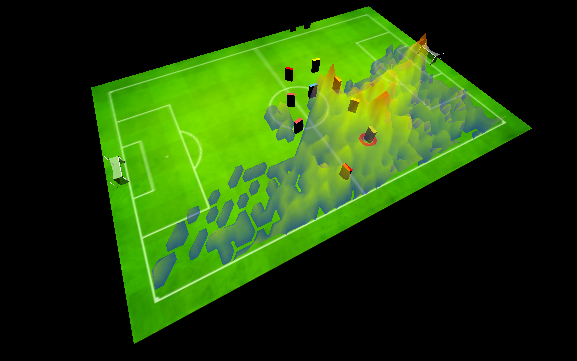
\includegraphics[width=.9\linewidth]{3dvis.png}
  \captionof{figure}{3D visualization with heatmap overlay}
  \label{fig:3dvis}
\end{minipage}%
\begin{minipage}{.5\textwidth}
  \centering
  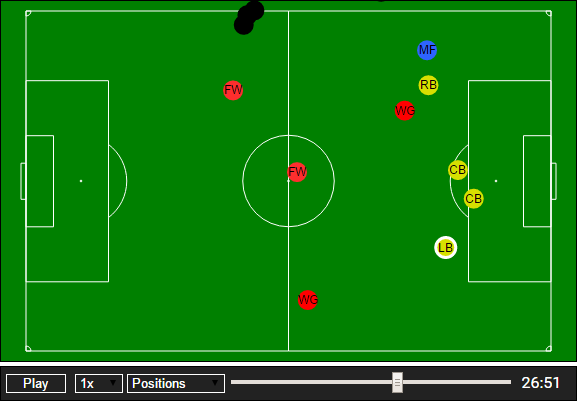
\includegraphics[width=.9\linewidth]{2dvis.png}
  \captionof{figure}{2D visualization with playback controls}
  \label{fig:2dvis}
\end{minipage}
\end{figure}

\end{document}